\chapter{Implementacija}\label{ch:impl}

Implementacija prati opisanu arhitekturu iz prethodnih poglavlja. 
Korisnički interfejs je zasnovan na arhitekturi jedne stranice, 
uz pomoć okruženja \textit{React}. Komunikacija između klijenta i servera 
je preko \textit{REST API}-a. Server je implementiran u arhitekturi
mikroservisa uz pomoć \textit{NestJS}. Za bazu podataka 
je izabrana \textit{PostgreSQL}. Za potrebe pravljenja zahteva za promenu 
na kodu, server komunicira preko \textit{GitHub} aplikacije. Autentikacija 
je implementirana preko \textit{OAuth} protokola, a za provajdera 
identiteta je izabran \textit{GitHub IdP}. Kao alat za \textit{CI/CD} se koriste 
\textit{GitHub Akcije}. 

Implementirano rešenje je nazvano \textit{Interpres}. Aplikacija je 
višejezična, odnosno može prikazati korisnički interfejs u više 
jezika. Za potrebe uređivanja prevoda je korišćen upravo \textit{Interpres}.

Izvorni kod je otvoren i može se naći na \url{https://github.com/enco164/interpres}.

\section{Komponente sistema}

Na slici \ref{fig:komponente} su prikazane komponente sistema kao i
njihove zavisnosti. Važno je napomenuti da, iako \textit{core} i 
\textit{user-management} mikroservisi koriste različite baze podataka,
baze se zapravo nalaze u istom sistemu za upravljanje bazama podataka. 
Ova odluka je donešena radi boljeg iskorišćenja resursa. 

\begin{figure}[h]
  \centering
  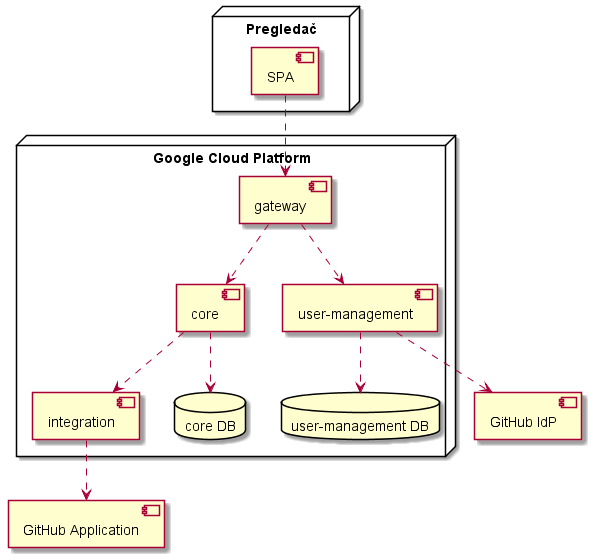
\includegraphics[width=0.7\textwidth]{komponente}
  \caption{Komponente sistema}
  \label{fig:komponente}
\end{figure}

U nastavku će biti opisana svaka komponenta, kao i njena 
zavisnost sa drugim komponentama.

\subsection{SPA}
Komponenta \textit{SPA} predstavlja klijentsku stranu aplikacije, implementiranu 
u stilu arhitekture jedne stranicne. Izgrađena je 
uz pomoć razvojnog okruženja \textit{React}. Za stilizovanje korisničkog 
interfejsa korišćena je biblioteka \textit{Material UI}. 

Kada se pokrene izgradnja \textit{React} projekta, artifakti koji se dobiju 
su \textit{HTML}, \textit{JavaScript} i \textit{CSS} fajlovi. Da bi korisnik dobio fajlove, 
potreban je veb server, i u te svrhe je izabran \textit{Nginx}.

Komponenta \textit{SPA} dobija podatke sa servera. Komunikacija sa serverom 
je preko protokola \textit{REST}, a ulazna tačka je mikroservis \textit{gateway}.

\subsection{Gateway}
Komponenta \textit{gateway} jedina "otvara kapiju" ka spoljnom svetu.
Ona služi da prihvati zahteve sa klijentske strane i prosledi ih 
drugim mikroservisima. S obzirom da ona predstavlja svojevrsnu "kapiju",
autentikacija je implementirana baš tu.

Provera pristupa se radi preko \textit{GitHub IdP}. Ako se korisnik 
prvi put prijavljuje na sistem, njegovi podaci o imenu i prezimenu će 
biti poslati mikroservisu \textit{user-management}. 

Komunikacija sa ostalim mikroservisima (\textit{core} i \textit{user-management})
se odvija preko protokola \textit{TCP} podržanog od strane \textit{NestJS}.

\subsection{User Management}
Cilj ove komponente je da se brine o podacima korisnika. Iako \textit{GitHub} 
predstavlja %TODO iyvor istine
izvor istine za podatke o korisniku, kao dobra praksa se 
pokazalo da ne treba zavisiti od ključeva nekih eksternih sistema. 
Ovde se konkretno misli na jedinstveni identifikator korisnika. Kao 
poboljšanje sistema, mogao bi da se implementira pristup sistemu preko 
nekog drugog provajdera identiteta. U tom slučaju može doći do kolizije 
ključeva, odnosno ne možemo da budemo sigurni da će različiti provajderi identiteta 
davati različite ključeve.

Pored brige o primarnim ključevima za korisnike, ovaj mikroservis služi 
i kao svojevrsna optimizacija. Naime, mnogo je brže kontaktirati 
mikroservis koji je u \textit{Kubernetes} klasteru nego neki eksterni 
servis.

\subsection{Core}
Mikroservis \textit{core} predstavlja srž aplikacije. On se bavi čuvanjem 
podataka o prevodima i o projektima. Tu se nalazi i poslovna logika za 
grupisanje i preslikavanje prevoda u strukturu koja je pogodna za 
klijentsku stranu aplikacije ili za mikroservis \textit{integration}.

\subsection{Integration}
Ova komponenta ima funkciju integracije sa sistemom za verzionisanje koda. 
Na zahtev mikroservisa \textit{core}, ona može preko \textit{GitHub Aplikacije}, 
da dohvati prevode sa repozitorijuma i da napravi \textit{Pull Request} sa 
novim izmenama. Ako bi se u budućnosti implementirala integracija sa nekim 
drugim sistemom za verzionisanje koda, ovaj mikroservis je pravo mesto za to.

\subsection{GitHub Application i GitHub IdP}
Da bi se napravila integracija sa \textit{GitHub}-om, za potrebe menjanja 
koda, potrebno je napraviti \textit{GitHub Application}. Aplikacija 
ustvari daje samo pristupne ključeve, a na programeru je dalje da implementira 
i postavi aplikaciju na neki server. Implementacija aplikacije u \textit{NodeJS} 
je preko \textit{GitHub}-ove biblioteke, nazvane \textit{octokit}. Preko ove 
biblioteke se dobija interfejs za sve akcije koje je moguće uraditi nad 
repozitorijumom. Dve glavne koje su implementirane su čitanje fajlova sa 
prevodima i pravljenje \textit{Pull Request}-a, i koriste se za uvoz i za 
izvoz prevoda.

\textit{GitHub IdP} je eksterna komponenta i služi kao provajder identiteta. 
Slično kao i za \textit{GitHub Application}, potrebna je samo registracija 
za dobijanje pristupnih ključeva kojima se pristupa interfejsu provajdera. 
Za implementaciju pristupa korićena je biblioteka \textit{Passport.js}, 
preporučena od strane \textit{NestJS}, koja ima implementaciju 
protokola \textit{OAuth2}, protokola koji koristi \textit{GitHub IdP}.

\section{Klijent}
Klijentski deo je izgrađen uz pomoć radnog okvira \textit{React}, a početna 
organizacija koda uz pomoć \textit{create-react-app}, preporučenog alata za 
generisanje \textit{React} projekta od strane \textit{Facebook}-a. 
Projekat je izgenerisan na jeziku \textit{Typescript}. 

Organizacija projekata je podeljena po funkcionalnostima, i one su 
\textit{auth} (odgovorna za autorizaciju), \textit{projects} (odgovorna za 
podešavanje projekta), \textit{import-export} (odgovorna za 
uvoz, odnosno izvoz prevoda) i \textit{translations} (odgovorna za uređivanje 
prevoda).

Sve \textit{React} komponente su pisane kao funkcijske komponente 
(eng. \textit{function components}) uz korišćenje kuka (eng. \textit{hooks}).
Programeri koji po prvi put koriste \textit{React} uglavnom nalaze da je 
ovako napisan kod nečitljiv jer deluje da je pomešana poslovna logika komponente 
sa prikazom korisničkog interfejsa. %TODO sl recenica
Iako se to može učiniti na početku, uglavnom je 
problem nepostojanja predloženog dizajna od strane autora biblioteke na 
zvaničnom sajtu. Poštovanjem pricipa da se sva poslovna logika %TODO cuva u kuki 
čuva u kuki, a da funkcijska komponenta koristi kuku i prikazuje sadržaj, 
postiže se veća čitljivost, razdvajaju se odgovornosti, lakše se testira 
automatskim testovima, a samim tim se kod lakše održava. 
Ovaj princip je prikazan na primeru koda \ref{code:primer}.
%TODO change listing caption label
\begin{listing}[H]
  \centering
\begin{minted}[ fontsize=\footnotesize ]{jsx}
// usePrimer.ts
export const usePrimer = () => {
  const [count, setCount] = useState(0);

  return {
    count,
    handleClick: () => setCount(count + 1),
  };
}

// primer.tsx
export const Primer = () => {
  const {count, handleClick} = usePrimer();

  return (
    <div>
      <p>Kliknuli ste {count} puta</p>
      <button onClick={handleClick}>
        Klikni me
      </button>
    </div>
  );
}
\end{minted}
\caption{Princip pisanja funkcijskih komponenata sa kukama}
\label{code:primer}
\end{listing}

Za upravljanje stanjem u aplikaciji korišćen je \textit{redux}. On radi 
po principu centralizovanog skladišta, što znači da njemu pristupaju sve 
komponente, odnosno da je on jedinstven %TODO iyvor istine 
izvor istine. Na taj način je 
napravljena sigurnost da podaci biti konzistentni i da neće biti particionisani.
Ako dve komponente zahtevaju isti podatak, one ga neće čuvati u svom stanju 
već će ga potraživati sa istog mesta.

\section{Server}
Svaki mikroservis je napravljen kao zasebna aplikacija i generisan uz pomoć 
\textit{NestJS} interfejsa za komandnu liniju. Ako neki mikroservis treba 
da zna za postojanje nekog drugog, informacija o lokaciji će biti prosleđenja 
kroz konfiguraciju, odnosno kroz promenljive iz okruženja. U konfiguraciji 
se pored toga čuvaju pristupni ključevi za \textit{GitHub Application}, 
\textit{GiHub IdP}, i lokacija i kredencijali za bazu podataka. Konfiguracija 
mikroservisa se učitava pri svakom podizanju.

Mikroservisi koji čuvaju stanje u bazi podataka su \textit{core} i 
\textit{user-management}. Kako \textit{NestJS} koristi u pozadini \textit{TypeORM}, 
iskorišćena je njegova funkcija migriranja baze podataka. Migracije služe 
za promenu sheme baze podataka u produkcionom okruženju. One osiguravaju da 
će prebacivanje na novu verziju sheme biti sigurno i da neće doći do gubitka 
podataka. Migracioni fajl sadrži klasu koja implementira 
\texttt{MigrationInterface}, a potrebno je implementirati dve metode: 
\texttt{up} i \texttt{down}. Prva služi da se baza migrira na višu 
verziju, a druga služi ako je u nekom slučaju potreban povratak na prethodnu. 
Unutar tih metoda treba napisati \textit{SQL} naredbe za migracije. Pored 
ručnog pisanja migracija, \textit{TypeORM} pruža i mogućnost generisanja 
migracionih klasa, jer može izračunati prethodni oblik modela, a odatle i 
razliku koju treba primeniti na bazu podataka kako bi podržala novi model. 

Stil pisanja koda na serveru je reaktivan uz \textit{rx.js} biblioteku koja
implementira obrazac "posmatrač". Kako je server napisan u stilu mikroservisa,
komunikacija među servisima je asinhrona, odnosno po principu 
"zahtev -- odgovor". To znači da dok neki servis čeka na odgovor drugog 
servisa, prvi može obavljati i neki drugi posao. Korišćenjem obrasca 
posmatrač se ova asinhronost lakše apstrahuje. Potrebno je napraviti zahtev 
i onda se pretplatiti na odgovor. Dok se čeka odgovor, pogram je slobodan da 
obavlja neki drugi posao. Kada odgovor stigne biće pozvana funkcija 
za obradu pretplate i tok izvršavanja će se nastaviti.
Pisanje reaktivnog koda je umnogome olakšano jer je i sam \textit{NestJS} 
napisan uz pomoć \textit{rx.js}. 

\section{Automatizacija}
Kontinualna integracija, isporučivanje i isporuka je implementirana uz 
pomoć \textit{GitHub}-a. Na glavnoj (\textit{"main"}) grani 
je postavljeno pravilo zaštite, odnosno onemogućeno je direkto slanje 
koda na tu granu. Za svaku izmenu koda potrebno otvoriti zahtev za 
promenu. Pored toga, postavljeno je pravilo da, grana koju treba spojiti 
na glavnu granu, mora sadržati sve izmene koje se nalaze na glavnoj grani.

Na događaj otvaranja novog zahteva za izmenu koda, pokreće se niz 
\textit{GitHub} akcija. Za klijentski deo i za svaki mikroservis 
se pokreće naredba izgradnje i naredba testiranja. Uz navedena 
ograničenja za spajanje grana, i sa ovom \textit{GitHub} akcijom, 
osigurava se da će spojeni kod biti istestiran pre spajanja. To znači da 
na glavnoj grani ne bi trebalo da se pojavi neka greška koja bi inače mogla 
da se otkrije testiranjem.

Kao i za zahtev za izmenu koda, kada se grana spoji u glavnu granu 
postoji niz \textit{GitHub} akcija, za svaku komponentu po jedna akcija.
Tu se izgrade \textit{Docker} slike koje se kasnije isporučuju na 
\textit{Docker} javni registar. Potom, kada su sve slike isporučene na 
\textit{Docker} registar, pokreće se \textit{GitHub} akcija koja započinje 
raspoređivanje na \textit{Kubernetes}.

\section{Produkciono okruženje}
Razne kompanije pružaju usluge iznajmljivanja računara u oblaku. Neki od 
poznatijih proizvoda su \textit{Amazon Web Services}, \textit{Microsoft Azure}
i \textit{Google Cloud Platform}. Sa druge strane, \textit{Kubernetes} je 
nezavisan od platforme. Iako ga je moguće instalirati i pokrenuti na sopstvenom 
serveru, taj posao je mukotrpan pa je pametnije izabrati neki proizvod gde se 
\textit{Kubernetes} može podići uz par klikova. 

Kako je \textit{Google} razvio \textit{Kubernetes}, pretpostavka je da je 
na \textit{Google Cloud Platform} uvek malo prednjači, pa je iz tog razloga 
on izabran za aplikaciju \textit{Interpres}.

Podešavanje na \textit{Google Cloud Platform} je jednostavno. Preko 
korisničkog interfejsa je potrebno napraviti klaster. Za klaster je 
potrebno izabrati tip virtualne mašine, kao i lokaciju servera na kojoj 
će ta virtualna mašina biti podignuta. Nadalje se sve može konfigurisati 
i preko komandne linije uz \textit{Kubernetes}-ov alat \texttt{kubectl}.
Preko ovog alata se izvršavaju komande sa pravljenje \textit{Pod}-ova.

Potrebno je napomenuti da se korišćenje \textit{Google Cloud Platform}-e,
naravno, naplaćuje. U trenutku pisanja ovog rada \textit{Google} za nove 
korisnike obezbeđuje besplatnih 300\$, koji su dovoljni za testiranje.
Svakako treba voditi računa prilikom podešavanja kako ne bi došlo do 
nepotrebnih troškova.

